\documentclass{standalone}
\usepackage{tikz}
\usetikzlibrary{patterns, positioning}


\begin{document}
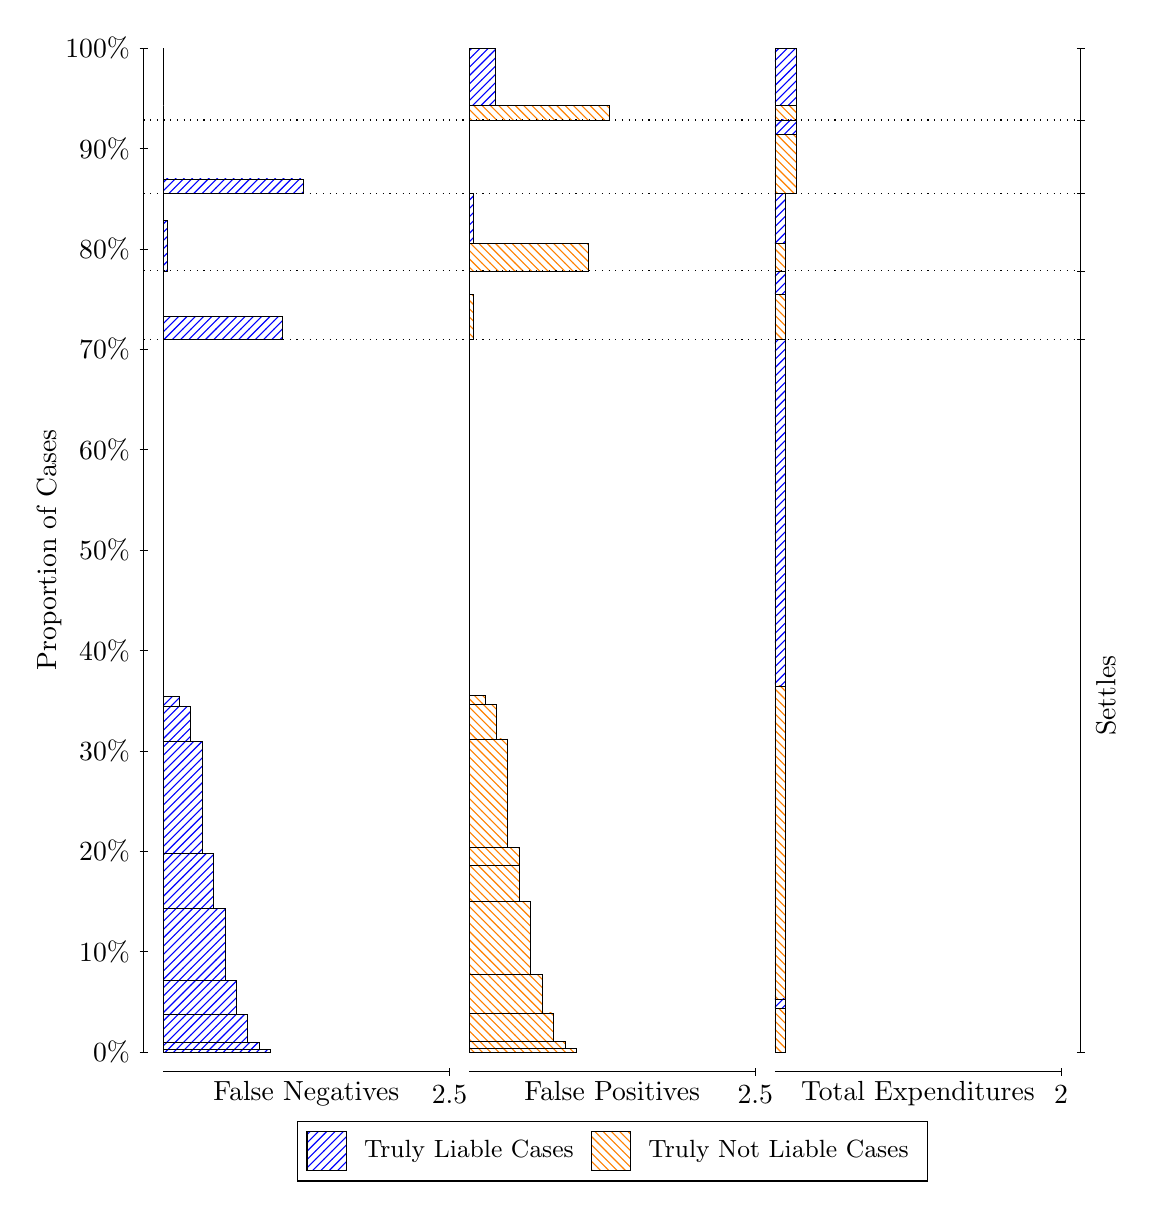
\begin{tikzpicture}
\draw[black, very thin] (1.5,1.75) -- (1.5,14.5);
\node[rotate=90, text=black, anchor=center] at (0.3, 8.125) {Proportion of Cases};
\draw[black, very thin] (1.45,1.75) -- (1.55,1.75);
\node[text=black, anchor=east] at (1.45, 1.75) {0\%};
\draw[black, very thin] (1.45,3.025) -- (1.55,3.025);
\node[text=black, anchor=east] at (1.45, 3.025) {10\%};
\draw[black, very thin] (1.45,4.3) -- (1.55,4.3);
\node[text=black, anchor=east] at (1.45, 4.3) {20\%};
\draw[black, very thin] (1.45,5.575) -- (1.55,5.575);
\node[text=black, anchor=east] at (1.45, 5.575) {30\%};
\draw[black, very thin] (1.45,6.85) -- (1.55,6.85);
\node[text=black, anchor=east] at (1.45, 6.85) {40\%};
\draw[black, very thin] (1.45,8.125) -- (1.55,8.125);
\node[text=black, anchor=east] at (1.45, 8.125) {50\%};
\draw[black, very thin] (1.45,9.4) -- (1.55,9.4);
\node[text=black, anchor=east] at (1.45, 9.4) {60\%};
\draw[black, very thin] (1.45,10.675) -- (1.55,10.675);
\node[text=black, anchor=east] at (1.45, 10.675) {70\%};
\draw[black, very thin] (1.45,11.95) -- (1.55,11.95);
\node[text=black, anchor=east] at (1.45, 11.95) {80\%};
\draw[black, very thin] (1.45,13.225) -- (1.55,13.225);
\node[text=black, anchor=east] at (1.45, 13.225) {90\%};
\draw[black, very thin] (1.45,14.5) -- (1.55,14.5);
\node[text=black, anchor=east] at (1.45, 14.5) {100\%};

\draw[black, very thin] (13.4,1.75) -- (13.4,14.5);
\draw[black, very thin] (13.35,1.75) -- (13.45,1.75);
\node[anchor=west] at (13.35, 1.75) {};
\draw[black, very thin] (13.35,10.797) -- (13.45,10.797);
\node[anchor=west] at (13.35, 10.797) {};
\draw[black, very thin] (13.35,11.669) -- (13.45,11.669);
\node[anchor=west] at (13.35, 11.669) {};
\draw[black, very thin] (13.35,12.657) -- (13.45,12.657);
\node[anchor=west] at (13.35, 12.657) {};
\draw[black, very thin] (13.35,13.586) -- (13.45,13.586);
\node[anchor=west] at (13.35, 13.586) {};
\draw[black, very thin] (13.35,14.5) -- (13.45,14.5);
\node[anchor=west] at (13.35, 14.5) {};

\draw[black, very thin, pattern color=blue, pattern=north east lines] (1.75,1.75) rectangle (3.1125,1.7866);
\draw[black, very thin, pattern color=blue, pattern=north east lines] (1.75,1.7866) rectangle (2.9672,1.8745);
\draw[black, very thin, pattern color=blue, pattern=north east lines] (1.75,1.8745) rectangle (2.8218,2.2233);
\draw[black, very thin, pattern color=blue, pattern=north east lines] (1.75,2.2233) rectangle (2.6765,2.664);
\draw[black, very thin, pattern color=blue, pattern=north east lines] (1.75,2.664) rectangle (2.5312,3.5722);
\draw[black, very thin, pattern color=blue, pattern=north east lines] (1.75,3.5722) rectangle (2.3858,4.2689);
\draw[black, very thin, pattern color=blue, pattern=north east lines] (1.75,4.2689) rectangle (2.2405,5.6903);
\draw[black, very thin, pattern color=blue, pattern=north east lines] (1.75,5.6903) rectangle (2.0952,6.1359);
\draw[black, very thin, pattern color=blue, pattern=north east lines] (1.75,6.1359) rectangle (1.9498,6.2705);
\draw[black, very thin, pattern color=orange, pattern=north west lines] (1.75,6.2705) rectangle (1.75,10.797);
\draw[black, very thin, pattern color=blue, pattern=north east lines] (1.75,10.797) rectangle (3.2578,11.095);
\draw[black, very thin, pattern color=orange, pattern=north west lines] (1.75,11.095) rectangle (1.75,11.669);
\draw[black, very thin, pattern color=blue, pattern=north east lines] (1.75,11.669) rectangle (1.8045,12.311);
\draw[black, very thin, pattern color=orange, pattern=north west lines] (1.75,12.311) rectangle (1.75,12.657);
\draw[black, very thin, pattern color=blue, pattern=north east lines] (1.75,12.657) rectangle (3.5303,12.838);
\draw[black, very thin, pattern color=orange, pattern=north west lines] (1.75,12.838) rectangle (1.75,13.586);
\draw[black, very thin, pattern color=orange, pattern=north west lines] (1.75,13.586) rectangle (1.75,13.767);
\draw[black, very thin, pattern color=blue, pattern=north east lines] (1.75,13.767) rectangle (1.75,14.5);
\draw[black, very thin, pattern color=orange, pattern=north west lines] (5.6333,1.75) rectangle (6.9958,1.7929);
\draw[black, very thin, pattern color=orange, pattern=north west lines] (5.6333,1.7929) rectangle (6.8505,1.8824);
\draw[black, very thin, pattern color=orange, pattern=north west lines] (5.6333,1.8824) rectangle (6.7052,2.2451);
\draw[black, very thin, pattern color=orange, pattern=north west lines] (5.6333,2.2451) rectangle (6.5598,2.7347);
\draw[black, very thin, pattern color=orange, pattern=north west lines] (5.6333,2.7347) rectangle (6.4145,3.662);
\draw[black, very thin, pattern color=orange, pattern=north west lines] (5.6333,3.662) rectangle (6.2692,4.1226);
\draw[black, very thin, pattern color=orange, pattern=north west lines] (5.6333,4.1226) rectangle (6.2692,4.3448);
\draw[black, very thin, pattern color=orange, pattern=north west lines] (5.6333,4.3448) rectangle (6.1238,5.7254);
\draw[black, very thin, pattern color=orange, pattern=north west lines] (5.6333,5.7254) rectangle (5.9785,6.1645);
\draw[black, very thin, pattern color=orange, pattern=north west lines] (5.6333,6.1645) rectangle (5.8332,6.2761);
\draw[black, very thin, pattern color=blue, pattern=north east lines] (5.6333,6.2761) rectangle (5.6333,10.797);
\draw[black, very thin, pattern color=orange, pattern=north west lines] (5.6333,10.797) rectangle (5.6878,11.37);
\draw[black, very thin, pattern color=blue, pattern=north east lines] (5.6333,11.37) rectangle (5.6333,11.669);
\draw[black, very thin, pattern color=orange, pattern=north west lines] (5.6333,11.669) rectangle (7.1412,12.015);
\draw[black, very thin, pattern color=blue, pattern=north east lines] (5.6333,12.015) rectangle (5.6878,12.657);
\draw[black, very thin, pattern color=orange, pattern=north west lines] (5.6333,12.657) rectangle (5.6333,13.406);
\draw[black, very thin, pattern color=blue, pattern=north east lines] (5.6333,13.406) rectangle (5.6333,13.586);
\draw[black, very thin, pattern color=orange, pattern=north west lines] (5.6333,13.586) rectangle (7.4137,13.767);
\draw[black, very thin, pattern color=blue, pattern=north east lines] (5.6333,13.767) rectangle (5.9603,14.5);
\draw[black, very thin, pattern color=orange, pattern=north west lines] (9.5167,1.75) rectangle (9.6529,2.3007);
\draw[black, very thin, pattern color=blue, pattern=north east lines] (9.5167,2.3007) rectangle (9.6529,2.4252);
\draw[black, very thin, pattern color=orange, pattern=north west lines] (9.5167,2.4252) rectangle (9.6529,6.4005);
\draw[black, very thin, pattern color=blue, pattern=north east lines] (9.5167,6.4005) rectangle (9.6529,10.797);
\draw[black, very thin, pattern color=orange, pattern=north west lines] (9.5167,10.797) rectangle (9.6529,11.37);
\draw[black, very thin, pattern color=blue, pattern=north east lines] (9.5167,11.37) rectangle (9.6529,11.669);
\draw[black, very thin, pattern color=orange, pattern=north west lines] (9.5167,11.669) rectangle (9.6529,12.015);
\draw[black, very thin, pattern color=blue, pattern=north east lines] (9.5167,12.015) rectangle (9.6529,12.657);
\draw[black, very thin, pattern color=orange, pattern=north west lines] (9.5167,12.657) rectangle (9.7892,13.406);
\draw[black, very thin, pattern color=blue, pattern=north east lines] (9.5167,13.406) rectangle (9.7892,13.586);
\draw[black, very thin, pattern color=orange, pattern=north west lines] (9.5167,13.586) rectangle (9.7892,13.767);
\draw[black, very thin, pattern color=blue, pattern=north east lines] (9.5167,13.767) rectangle (9.7892,14.5);
\draw[black, dotted] (1.5,10.797) -- (13.4,10.797);
\draw[black, dotted] (1.5,11.669) -- (13.4,11.669);
\draw[black, dotted] (1.5,12.657) -- (13.4,12.657);
\draw[black, dotted] (1.5,13.586) -- (13.4,13.586);
\draw[black, very thin] (1.75,1.5) -- (5.3833,1.5);
\node[text=black, anchor=north] at (3.5667, 1.5) {False Negatives};
\draw[black, very thin] (5.3833,1.45) -- (5.3833,1.55);
\node[text=black, anchor=north] at (5.3833, 1.45) {2.5};

\draw[black, very thin] (5.6333,1.5) -- (9.2667,1.5);
\node[text=black, anchor=north] at (7.45, 1.5) {False Positives};
\draw[black, very thin] (9.2667,1.45) -- (9.2667,1.55);
\node[text=black, anchor=north] at (9.2667, 1.45) {2.5};

\draw[black, very thin] (9.5167,1.5) -- (13.15,1.5);
\node[text=black, anchor=north] at (11.333, 1.5) {Total Expenditures};
\draw[black, very thin] (13.15,1.45) -- (13.15,1.55);
\node[text=black, anchor=north] at (13.15, 1.45) {2};

\node[text=black, centered, rotate=90] at (13.72, 6.2733) {Settles};





\draw (7.449999999999999,1.5) node[draw=none] (baseCoordinate) {};
\begin{scope}[align=center]
        \matrix[scale=0.5, draw=black, below=0.5cm of baseCoordinate, nodes={draw}, column sep=0.1cm]{
            \node[rectangle, draw, minimum width=0.5cm, minimum height=0.5cm, pattern color=blue, pattern=north east lines] {}; &
            \node[draw=none, font=\small, text=black] (B) {Truly Liable Cases}; &
            \node[rectangle, draw, minimum width=0.5cm, minimum height=0.5cm, pattern color=orange, pattern=north west lines] {}; &
            \node[draw=none, font=\small, text=black] (B) {Truly Not Liable Cases}; \\
            };
\end{scope}

\end{tikzpicture}
\end{document}